\chapter{Introduction}
\section{Motivation}
The development towards greener propulsion systems have played a major part of
the automotive industry during the 21st century. There have been numerous
incentives to push engineering towards less energy consuming propulsion
alternatives. One of these incentives is Shell Eco-marathon (SEM), where
university students from all over the world come together to compete in fuel
efficiency. Naturally there should be a contribution from KTH and the complexity
of the system makes the collaboration between the masters in Mechatronics,
Internal Combustion Engine and Machine Design very wise. It also opens for collaborations from other departments such as lightweight constructions. By combining these
engineering branches the entire system boundary is covered and there is a good
overlap between the programs in the boundary areas. The Mechatronic part of the
project is a substantial part, which makes the collaboration between the
Advanced Course in Mechatronics and the Integrated Transport Research Lab (ITRL)
a really good fit for the project.

\section{Shell Eco-Marathon}
Shell Eco-Marathon is a yearly competition for students to compete with fuel
efficient, custom made, vehicles~\cite{SEM_web}. The competition dates back to
1939 and have been in different locations trough out the years. SEM is split
into three regional championships, Europe, Americas and Asia with a World Final
for the winners in the different classes. There are two main class divisions,
\textit{Prototype} and \textit{UrbanConcept}. There are also sub classes within
the main classes based on what fuel/energy type the vehicle uses. Each fuel has
an assigned energy value~\cite{semrules16c1} which makes different fuel types
comparable.

\subsection{Urban Concept Vehicle}\label{UCV}
Elba competes in the UrbanConcept class and is what is called a UrbanConcept
Vehicle (UCV). The vehicles in this class have an appearance closer to today's
production type passenger cars. The cars in the class have to be built in
accordance with the class specific rules that dictates everything from steering
and controls to propulsion and safety. UCVs must have some common production
car features as wind shield wiper, turn signals, horn headlights etc. Vehicles
competing in this group is also required ``stop and go'' each lap, which means
that once every lap the vehicle needs to do a full stop. This is to further
increase the resemblance to city driving.

\subsection{London Track}
All vehicles drive the same amount of laps, 8 in 2016(\cite{semrules16c2}),
which equals 17.9 kilometres. Compared to earlier tracks the London track has a
steeper height profile. To climb the steepest part of the track the vehicles
must deliver larger amounts of torque than previous years (this is true for
Elba). The height profile of the track can be seen in
Figure~\ref{fig:introduction_londontrack}.
\begin{figure}[H]
    \centering
    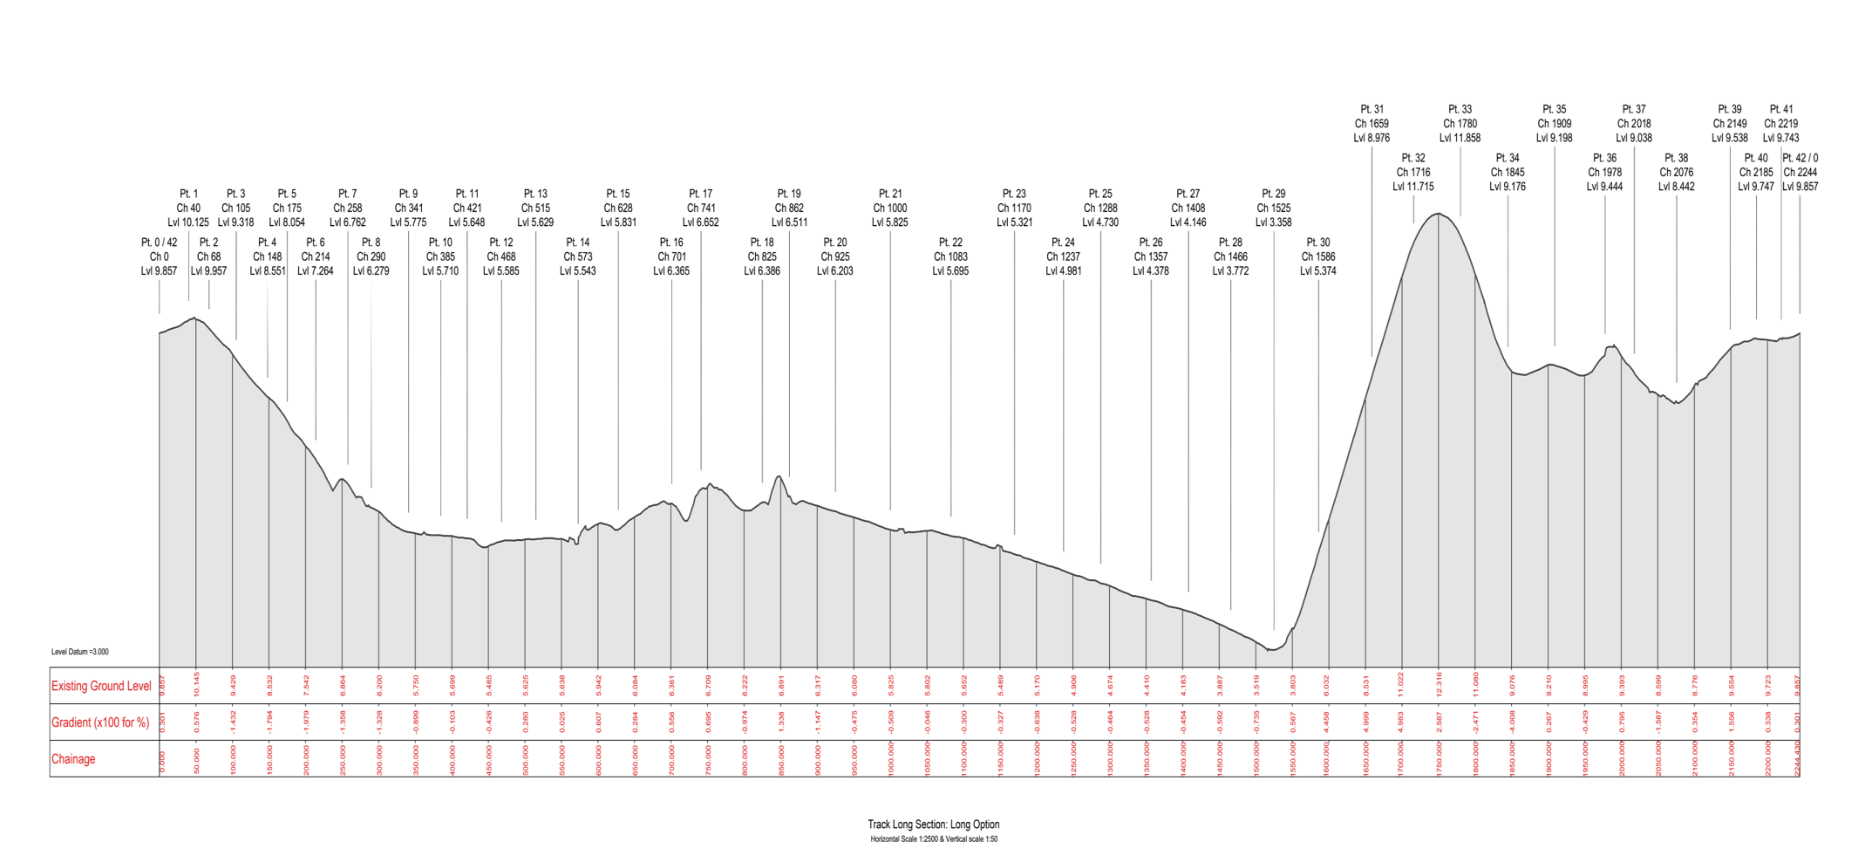
\includegraphics[width=\textwidth]{./img/introduction_londontrack.png}
    \caption{Height profile of the London
    track.}\label{fig:introduction_londontrack}
\end{figure}

\subsection{Inspections}
Before any vehicle is allowed on the track it must first pass two inspections,
the safety inspection and the technical inspection. The safety inspection covers
issues related to the safety of the driver, personnel and surrounding cars. 
The technical inspection covers how the vehicle compiles to the rules,
specifically energy usage. This ensures that the car does not use power from the
auxiliary power source to propel the vehicle in any way.

Simply passing these inspections is nothing that many teams take lightly and it
can be the main goal for many of the teams attending SEM\@. This means that
if the car does not change year-to-year it is often easier to get the car to
race the next year.

\section{Purpose}
If one wishes to perform well in Shell Eco-Marathon optimising the speed the car should have on the track could improve performance. 
This is also something that is interesting for the industry and is not use in current cars when using autimatic speed thingys. This would both save money and the environment due to the reduced fuel consumption.

One goal the optimisation is to improve result at SEM\@. Therefore a car, in competition shape, has to be maintained. The car has to be updated to comply whit the current SEM-rules and also simply to be cemt in a drivable state. The car is also seen as a platform for students to test ideas and perform research. Various parts of the car have already been developed as bachelors thesis's and the optimisation will be improved as a part of a master thesis. The car enables students to try to solve both complex construction and design tasks, such as the unique clutch or the laminate door, and experiment with different optimisation strategies in a real world case. Appearing and performing well with the car is the main way to get sponsorship deals to support the project, both with parts and with money to cover travel and transportation costs.

But to be able to do all this test has to be carried out with as little overhead (time, track, transportation etc.) as possible. Also the actual competition track is located in London (and it only exists during the event), so there is no option to go there and test. This is the motivation behind the testrig. Other teams competing in SEM uses these machines to test the car while standing still, but KTH EcoCars had no machine like this. The testrig solves several practicalities for KTH EcoCars and is therefore not only beneficial for the car that was worked on, Several problems had to be solved for it to work: is must supply the torque demanded, is must simulate the forces the car is exposed to, and is has to handle supply of energy and regenerated energy created when braking the car.

%Requirements Engineering
\section{Requirement engineering}
In a complex system, there are many stakeholders, both internal and external.
The requirements are meant to capture the needs of the users and convey them to
the developers~\cite{ibm_req}. It is important that the requirements are
unambiguous~\cite{ibm_req, rupp2014} in order for there to be no room for
interpretation. Since natural language is ambiguous by nature, there are
standardized frameworks and templates to improve the quality of the
requirements~\cite{rupp2014}. 

\subsection{User and system requirements}\label{sec:req_usr_sys}
Requirements can be organized into two categories, User and System requirements.
These differ in a number of ways, both in their nature and how they are
procured. A project design often starts with a demand or need from a customer or user.
These needs can be seen as the goal for the project to fulfil and are of a high
level, abstract nature. They are captured from the future users of the system
and are expressed in the users language. In essence, the User requirements
describe the problem that is to be solved by the system~\cite{ibm_req}. 

When the User requirements are set, these need to be condensed into technical
requirements that the developers can work towards, these are the System
requirements. They define what the system and its sub-systems is supposed to do
an it is the developers that own these requirements. They are therefore also
responsible for that these in turn fulfill the User requirements~\cite{ibm_req}.

\subsection{Requirement formulation}
As described in Section~\ref{sec:req_usr_sys}, it is important that requirements
are clear and unambiguous. By using standardized templates when expressing the
requirements, there is a framework where it is clear an unanimous what a word or
phrase means.  This greatly increases the quality of the
requirements\cite{rupp2014}.  By using a template for the structure of a
requirement, it is ensured that all parts needed are in the requirement.
Rupp~\cite{rupp2014} gives a template on how to formulate a
requirement, which can be seen in Figure~\ref{fig:req_template}.
\begin{figure}[H]
    \centering
    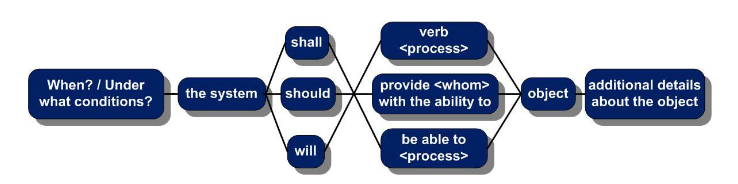
\includegraphics[width=\textwidth]{./img/introduction_req_template.PNG}
    \caption{Requirement formulation template.}\label{fig:req_template}
\end{figure}
It is also important to realize that in a complex system, there are many
relationships between stakeholders and requirements~\cite{ibm_req}. A ange in
one requirement may affect several other requirements. Therefore, it is
important to have a requirement software that makes it easy to track the
dependencies between the different requirements.

% More info on requirement system

% Draft on design desitions
\section{Design Decisions}
When developing a product there might be multiple solutions to a problem, 
where the solutions might (or might not) fulfil relevant requirements. 
The entire team where involved in subgroup decisions which meant they had to motivate
the different alternatives before one was chosen. These decisions all related to the 
car and the competition, so they had to follow the cars requirements derived from the rules.

Decisions also had to made for the optimisation and the testrig. 
